\section{Результаты}

В эксперименте использована установка, состоящая из калориметра, представляющего собой стеклянную цилиндрическую трубку с двойными стенками, запаянную с торцов. Из пространства между стенками откачан воздух до высокого вакуума ($10^{-5}$ торр). В калориметр встроен нагреватель - нихромовая проволока. Воздух прокачивается через калориметр с помощью компрессора. 

Более подробное описание установки см. в \nameref{Приложение 1}.

Мощность нагрева нихромовой проволоки вычисляется по значениям напряжения и тока, текущего через нее. Напряжение $U$ и ток $I$ регистрируются цифровыми мультиметрами. Таким образом
\begin{equation}
    N = U \cdot I
\end{equation}

Для определения разности температур $\Delta T$ воздуха на концах калориметра служит медно-константановая термопара. Один спай термопары расположен в струе воздуха, входящего в калориметр, и находится при комнатной температуре $T_0 = \SI{22.2}{\celsius}$, а второй в струе выходящего нагретого воздуха. Константановая проволока термопары расположена внутри калориметра, а медные проводники подключены к цифровому вольтметру. Напряжение $E$ на вольтметре пропорционально разности температур $\Delta T$ спаев
\begin{equation}
    E = \beta\Delta T \label{eq: E}
\end{equation}


(температура измеряется с помощью нагревательной проволоки, используемой как термопара, подробное описание определения температуры по формулам -> в приложение)
(аналогично для расхода и мощности нагревателя)

$\beta = 40.7 \frac{\text{мкВ}}{\celsius}$ - чувствительность термопары в рабочем диапазоне температур $20-30\celsius$.

Массовый расход $q$ воздуха, проходящего через калориметр, вычисляется через объемный расход следующим образом
\begin{equation}
    q = \rho_0\frac{\Delta V}{\Delta t} \label{eq: q}
\end{equation}
$\rho_0$ - плотность воздуха при комнатной температуре и атмосферном давлении $P_0 = 101600 \text{Па}$. Из уравнения Менделеева-Клапейрона: $\rho_0 = \frac{\mu P_0}{RT_0}$, где $\mu = 29 \frac{\text{г}}{\text{моль}}$ - средняя молярная масса сухого воздуха. Подставляя выражение для $\rho_0$ в $\eqref{eq: q}$, получаем
\begin{equation}
    q = \frac{\mu P_0}{RT_0}\frac{\Delta V}{\Delta t} \label{eq: q_2}
\end{equation}
Объем $\Delta V$ воздуха, проходящего через калориметр, измеряется газовым счетчиком (см. описание экспериментальной установки в \nameref{Приложение 1}). Время $\Delta t$ прохождения некоторого объема $\Delta V$ воздуха измеряется секундомером.

Перед каждой серией измерений зависимости $N$ от $\Delta T$ при фиксированном расходе воздуха калориметр был охлажден до комнатной температуры. Компрессор включен, кран К открыт до максимального расхода воздуха, источник постоянного тока выключен. 

Чтобы в процессе измерений величина $\Delta T$ равномерно увеличивалась от 2 до $\SI{10}{\celsius}$, была оценена величина тока $I_0$ нагревателя, требуемая для нагрева воздуха на $\SI{1}{\celsius}$. Способ вычисления $I_0$ описан в \nameref{Приложение 2}. Таким образом, чтобы нагреть воздух на $\Delta T = 2\celsius$, нужно пропустить через нить ток $I \approx 2I_0$.

По измеренным зависимостям $N(\Delta T)$ для двух расходов воздуха построены графики. Результаты измерения представлены на рисунке
\begin{center}
    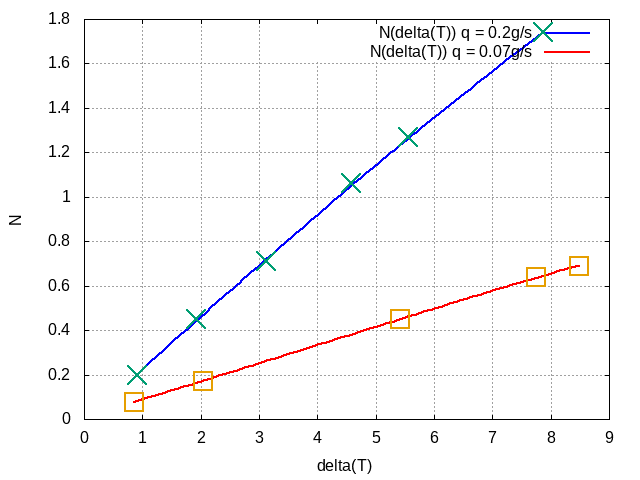
\includegraphics[width=0.9\textwidth]{img/graph4 (2).png}
    
    Графики зависимости $N(\Delta T)$
\end{center}
(добавить подписи к графикам, непонятно что такое $N, \Delta T$)

Графики, изображенные на рисунке, являются линейными. Значит, предположение о том, что при небольшом нагреве ($\Delta T \ll T_0$) мощность $N_\text{пот}$ тепловых потерь пропорциональна разности температур $\Delta T$, оказалось верным.

По методу наименьших квадратов определены коэффициенты $k$ наклона прямых. Таблица значений $k$ при двух расходах $q$ представлена в \nameref{Приложение 4}.

Используя данные из таблицы 3 (см. \nameref{Приложение 4}) построили график зависимости $k(q)$ 

\begin{center}
    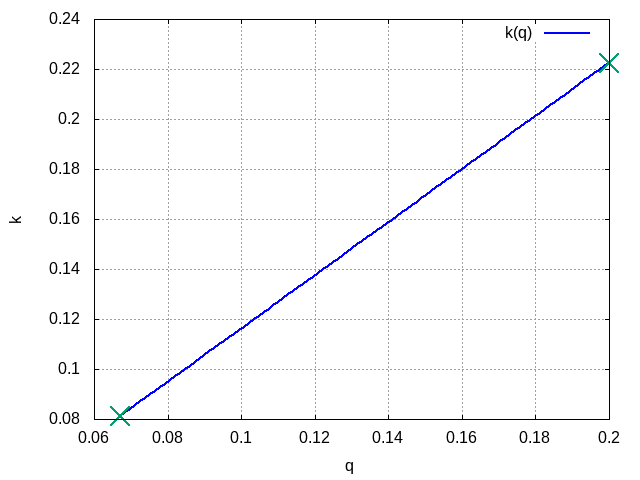
\includegraphics[width=0.9\textwidth]{img/graph6 (1).png}
    
    Графики зависимости $k(q)$
\end{center}

Из графика видно, что $k$ линейно зависит от расхода $q$ и является возрастающей функцией. При увеличении расхода $q$ воздуха, прокачиваемого через калориметр, увеличивается масса $\Delta m = q\Delta t$ воздуха, которую необходимо нагреть на температуру $\Delta T$ за время $\Delta t$. Из этого следует, что увеличивается количество теплоты, которое нужно передать воздуху за время $\Delta t$, чтобы нагреть его на температуру $\Delta T$. Значит, увеличивается $k = \frac{Q}{\Delta T \Delta t} = \frac{N}{\Delta T}$.

С помощью метода наименьших квадратов определили удельную теплоемкость $c_p$ при постоянном давлении как угловой коэффициент графика $k(q)$ и коэффициент $\alpha$ в выражении \eqref{eq: N(delta T)} как точку $(0;\alpha)$ пересечения графика с осью $k$.
\begin{center}
    $c_p = (1063 \pm 13)\frac{\text{Дж}}{\text{кг} \cdot \text{К}}$

    $\alpha = (19 \pm 1)\cdot 10^{-3}\frac{\text{Дж}}{\text{K}}$
\end{center}

По полученному коэффициенту $\alpha$ была рассчитана доля мощности тепловых потерь от мощности нагревателя при каждом расходе воздуха.
\begin{equation}
    \frac{N_{\text{пот}}}{N} = \frac{\alpha\Delta T}{(c_p q + \alpha)\Delta T} = \frac{\alpha}{k}
\end{equation}
Результаты вычислений приведены в таблице 4 (см. \nameref{Приложение 5}).


Согласно таблице 4 (см. \nameref{Приложение 5}) доля $\frac{N_{\text{пот}}}{N}$ увеличивается при уменьшении расхода $q$ воздуха. Действительно, при уменьшении расхода увеличивается время теплообмена воздуха, текущего через калориметр, с окружающей средой. Из этого следует, что увеличивается энергия, расходующаяся на нагрев окружающей среды. Значит  $\frac{N_{\text{пот}}}{N}$ возрастает.